\documentclass[12pt]{article}
\parindent0em
\parskip 1ex plus 0.4ex minus 0.4ex

\usepackage[a4paper,vmargin=30mm,hmargin=25mm]{geometry}
\usepackage{polyglossia}
\setdefaultlanguage{german}
\usepackage{caption}
\usepackage{fontspec}
\usepackage{lipsum}
\usepackage{xcolor}
\usepackage{listings}
\usepackage{amssymb}
\usepackage{hyperref}
\usepackage{graphicx}

\definecolor{lstbackground}{rgb}{0.95,0.95,1}      % hellgruener Rahmen
\lstset{language=Python}

\lstset{
  basicstyle=\small\ttfamily,
  backgroundcolor=\color{lstbackground},
  keywordstyle=\bfseries\ttfamily\color{blue},
  stringstyle=\color{orange!50!black}\ttfamily,
  commentstyle=\color{gray}\ttfamily,
  showstringspaces=false,
  flexiblecolumns=false,
  tabsize=4,
  numbers=left,
  numberstyle=\tiny,
  numberblanklines=true,
  stepnumber=1,
  numbersep=10pt,
  xleftmargin=15pt,
  literate=%
  {Ö}{{\"O}}1
  {Ä}{{\"A}}1
  {Ü}{{\"U}}1
  {ß}{{\ss}}1
  {ü}{{\"u}}1
  {ä}{{\"a}}1
  {ö}{{\"o}}1
  {~}{{\textasciitilde}}1
}

\begin{document}

\begin{center}
  \textbf{\LARGE Sichere Programmierung} \\[1ex]%
  \textbf{\Large Projekt 2}\\[2ex] %
  Julian Sobott \\ %
  (76511) \\ %
  David Sugar \\ %
  (76050) \\ %
  
\end{center}

% ****************************************************************************
\section{Zu Aufgabe 1}
% ****************************************************************************
\subsection{a)}
Zu beginn der \texttt{main()} Funktion wird eine \texttt{unsigned int} Variable, i, deklariert, jedoch nicht initialisiert, d.h. bis auf wenige Ausnahmen $i \in \{0..2^{32}-1\}$.

Danach wird die Variable im Kopf der darauf folgenden For-Schleife mit 0 initialisiert. Die Schleife inkrementiert die Variable i am Ende jedes Schleifendurchlaufs und tritt erneut in die Schleife ein, solange i kleiner 20 ist.
Innerhalb der Schleife wird der Wert von i, zum jeweiligen Zeitpunkt, formatiert mithilfe von \texttt{printf()} in der Standardausgabe ausgegeben. Dabei werden immer 2 Stellen ausgegeben, dies wird über \texttt{"\%2d"} realisiert.

\textbf{Potentielles Problem: Es sollte \texttt{"\%2u"} verwendet werden, da \texttt{d} für die Formatierung von signed Integern verwendet wird.} In diesem Fall spielt die Formatierung aber keine Rolle.

\subsection{b)}
Bild \ref{fig:aufgabe1b} zeigt die Ausgabe des Programms.
\begin{figure}[h]
	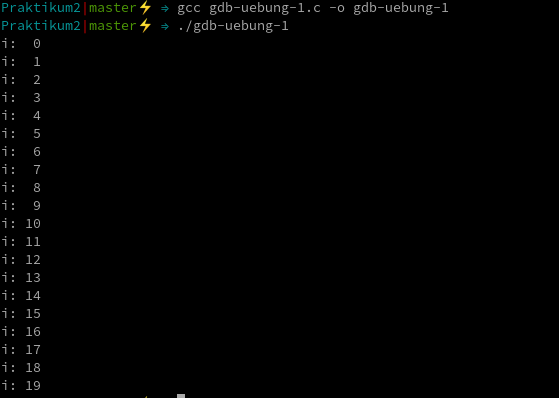
\includegraphics[scale=0.9]{Pictures/aufgabe1b.png}
	\caption{Ausgabe von gdb-uebung-1.c}
	\label{fig:aufgabe1b}
\end{figure}

\subsection{c)}
\begin{lstlisting}
	<+8>:	mov    DWORD PTR [rbp-0x4],0x0
    <+15>:	jmp    0x40113b <main+41>
    <+17>:	mov    eax,DWORD PTR [rbp-0x4]
    <+20>:	mov    esi,eax
    <+22>:	mov    edi,0x402004
    <+27>:	mov    eax,0x0
    <+32>:	call   0x401030 <printf@plt>
    <+37>:	add    DWORD PTR [rbp-0x4],0x1
    <+41>:	cmp    DWORD PTR [rbp-0x4],0x13
    <+45>:	jbe    0x401123 <main+17>
\end{lstlisting}

Für die Variable i wird Speicher auf dem Stack alloziert, die Anfangsadresse ist dabei \texttt{rbp-0x4}.

In Zeile <+8> wird i mit 0x0 initialisiert. Danach springt das Programm unbedingt in Zeile <+41>. Hier befindet sich nun die Überprüfung, ob die Schleife verlassen wird, d.h. $ i \ge 0x14 $, oder ein weiterer Schleifendurchlauf gestartet wird. Dazu wird in Zeile <+41> i mit 0x13 verglichen. Ist der Wert kleiner oder gleich 0x13 wird in Zeile <+17> gesprungen und damit ein weiterer Schleifendurchlauf gestartet. Andernfalls wird die nächste Instruktion ausgeführt und damit die Schleife verlassen.

In Zeile <+17> und <+20> wird der Wert von i, vom Speicher in das \texttt{esi} Register geladen. In der darauf folgenden Zeile wird die Adresse des Formatierungsstrings ("i: \%2d\\n") ( 0x402004 ) in \texttt{edi} geladen.

\begin{lstlisting}
gef➤  x/s 0x402004
0x402004:	"i: %2d\n"
\end{lstlisting}

Weiterhin wird \texttt{eax} wieder auf 0x0 zurückgesetzt. Danach wird \texttt{printf()} mit den in \texttt{edi} und \texttt{esi} geladenen Parametern aufgerufen. Schlussendlich wird i inkrementiert und daraufhin wieder verglichen (<+41>).

\subsection{d)}

\newcommand{\imageseries}[1]{
\begin{center}
   \includegraphics[width=\textwidth]{Pictures/a1d_#1.png}
	\captionof{figure}{#1. Ausgabe von gdb-uebung-1.c}
\end{center}
%\begin{figure}[ht!]
%	\includegraphics[scale=0.5]{Pictures/a1d_#1.png}
%	\caption{#1. Ausgabe von gdb-uebung-1.c}
%	\label{fig:a1d_#1}
%\end{figure}
}

In dieser Aufgabe geht es nun darum das Programm \texttt{gdb-uebung-1.c} in gdb auszuführen. Im folgenden wird der Ablauf durch Screenshots und entsprechende Erklärungen beschrieben.

\imageseries{1}


1. Hier beginnt die \texttt{main} Funktion. Als erstes wird der \texttt{rsp} Zeiger, welcher auf den Stack zeigt, um \texttt{0x10} verschoben, um entprechen Platz auf den Stack zu allozieren.

\imageseries{2}

2. Initialisieren der Variable i  mit 0x0.

\imageseries{3}

3. Unbedingter Sprung in Zeile <main+41>.

\imageseries{4}

4. Ausgabe von i. (Adresse: Wert). Der Wert wird in Dezimal ausgegeben.

Schritte bis zur nächsten Zeile wurden übersprungen, da sie in Aufgabe 1 b) ausführlich erklärt wurden.

\imageseries{5}

5. Der bedinge Sprung \texttt{jbe} (jump below or equal) wird genommen, da $ 0x0 \le 0x13$. Das heißt, das Programm spring zu <main+17>.

\imageseries{6}

6. Schreiben des Wertes von i in eax und eax dann in esi, um i als Parameter an die \texttt{printf} Funktion zu übergeben.

\imageseries{7}
\imageseries{8}

7.+ 8. Aufrufen der \texttt{printf} Funktion mit i=0. Übergeben wird in rsi und rdi der Wert von i und ein pointer auf den format string. Dieser Aufruf führt zu folgender Ausgabe auf dem Standardoutput:

\begin{lstlisting}
i: 0
\end{lstlisting}

\imageseries{9}

9. Hier wird der Wert von i nun um eins erhöht.

\imageseries{10}

10. Nach der ausführung ist der Wert 1.

\imageseries{11}

11. Als nächstes wollen wir das Programm bis zum letzten Durchlauf laufen lassen und dort dann einen Breakpoint setzen. Als erstes geben wir uns hierfür die Adresse für i aus. Diese wird benötigt, da der Conditional Breakpoint nur stoppen soll, wenn i einen bestimmten Wert hat. In der nächsten Zeile setzen wir den Conditional Breakpoint in die Zeile wo der bedingte Sprung ist (<main+45>). Als Bedingung geben wir an, dass der Wert von i gleich 0x13 sein soll. Wie auch in C müssen Adressen jeweils mit dem * dereferenziert werden. Am Ende wird noch kontrolliert ob der breakpoint richtig gesetzt wurde.

\imageseries{12}

12. Lassen wir das Programm nun mit continue (c) laufen, sehen wir alle Schleifendurchläufe mit den entsprechenden Ausgaben. Die letzte Ausgabe ist 18 (0x12).

\imageseries{13}

13. Der bedingte Sprung wird ein letztes Mal genommen, da der Wert von i gleich 19 (0x13) ist.

\imageseries{14}

14. Die Schleife ist eine letztes Mal durchgelaufen wie erwartet und hat noch die 19 ausgegeben. Wenn wir nun aber an dem bedingten Sprung angkommen wird dier nicht mehr genommen, da die Bedingung nicht mehr zutrifft (i = 0x14 und somit glit nicht mehr i <= 0x13).

\imageseries{15}

15. Anstatt an <main+17> zu springen, wurde zur nächsten Anweisung gesprungen <main+47>. Somit wurde die Schleife verlassen. Hier wird noch die 0 als Rückgabewert gespeichert. 

\imageseries{16}

16. Mit continue (c) lassen wir das Programm zuende durchlaufen und es wird normal beendet.


% ****************************************************************************
\section{Zu Aufgabe 1}
% ****************************************************************************
\subsection{a)}

Anlyse des Programs \textit{gdb-uebung-2.c}

\lstinputlisting{../gdb-uebung-2.c}

Das Programm besteht aus drei Hilfsfunktionen \texttt{f}, \texttt{g}, \texttt{h}, die jeweils 2 int's als Eingabe bekommen und mit Grundrechenarten ein Ergebnis berechnen und zurück geben. Die Berechnungen scheinen willkürlich sein. 

In der \texttt{main} Funcktion, werden zuerst drei int's \texttt{a, b, c} initialisiert werden. Daraufhin wird in einem geschachtelten Funktionsaufruf der Wert von \texttt{c} berechnet. In den Funktionsaufrufen, werden die Rückgabewerte einer Hilfsfunktion immer direkt an die nächste Funktion, als Parameter, übergeben. Am Ende wird durch ein Aufruf der \texttt{printf} Funktion ein formatierter String mit den Werten von den Variablen ausgegeben.


\subsection{b)}

Bild \ref{fig:aufgabe2b} zeigt die Ausgabe des Programms.
\begin{figure}[h!]
	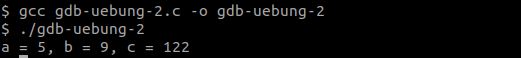
\includegraphics[width=\textwidth]{Pictures/a2b.png}
	\caption{Ausgabe von gdb-uebung-2.c}
	\label{fig:aufgabe2b}
\end{figure}


Wie erwartet sind die Werte von \texttt{a, b} unverändert zur ursprünglichen Initialisierung. Nur \texttt{c} hat den den neuen Wert, den es zugewiesen bekommen hat.

\subsection{c)}

\subsubsection{Reihenfolge der Funktionsaufrufe}

Die Reihenfolge wurde herausgefunden, indem in gdb mit s immer der nächste Schritt ausgeführt wurde. Hierfür wurde das Programm mit Debug Informationen compiliert (Option -g bei gcc).


\begin{enumerate}
\item \texttt{h(9, 5)} (2. h)
\item \texttt{h(5, 9)} (1. h)
\item \texttt{g(5, 314)}
\item \texttt{f(-692, 314)}
\end{enumerate}

Interessant bei der Ausführung ist, dass bei dem Aufruf von \texttt{f} zuerst der 2. Parameter (\texttt{h} )ausgewertet wird und dann erst der 1. (\texttt{g}).

Stack Frames: TODO

https://stackoverflow.com/questions/2770889/how-can-i-examine-the-stack-frame-with-gdb


For the current stack frame:

    info frame lists general info about the frame (where things start in memory, etc.)
    info args lists arguments to the function
    info locals lists local variables stored in the frame






















\end{document}



%%% Local Variables: 
%%% TeX-PDF-mode: t
%%% TeX-master: t
%%% coding: utf-8
%%% mode: latex
%%% TeX-engine: xetex
%%% End: 
